\section{Cluster dispersion and separability} \label{sec:BG:dataSeparability}
The EMG-signal for each movement class acquired from the subjects forms clusters of multidimensional data points. The lower the dispersion of the individual movement class clusters is, the more distinguishable the movements are, and the classifier will recognize the movement classes with higher accuracy. Additionally, a higher distance between cluster centroids will facilitate a higher classification accuracy further. This can be used to evaluate the users' ability to improve in performing distinguishable movements between sessions. This section describes how to calculate the cluster dispersion and separability of clusters. \\

\subsection{Distance measure} \label{sub:BG:distanceMeasure}
To calculate cluster dispersion, the centroid of multidimensional clusters must be calculated as in:

\begin{equation} \label{eq:centroid}
C = \Bigg[ \frac{\sum\limits_{n=1}^{N}x_{n},y_{n},~...~k_{n}}{N} \Bigg]
\end{equation}

Where $C$ is the centroid, $n$ is the number of data point in a dimension, $N$ is the total number of data points in a dimension and $k$ is the number of dimensions. To calculate cluster dispersion, the Euclidean distance (ED) from data point $p$ to the corresponding cluster $q$ is computed: %The ED is the length of the a line segment connecting points, in this case in form of data point $p$ and cluster centroid $q$, and is calculated as:

\begin{equation} \label{eq:euclidiandistance}
ED(p,q) = \sqrt{(p_1-q_1)^2 + (p_2-q_2)^2~+~...~+ (p_k-q_k)^2}
\end{equation} 

This procedure is performed for all data points in a cluster, from which the average ED is calculated to obtain the dispersion of a cluster. To get a general impression of the cluster dispersion of all classes, the average of all cluster dispersions are calculated.\\
To calculate the cluster separability, the ED between cluster centroids is calculated. The average of the distance between all clusters are then calculated to get a general impression of the cluster separability.   

%Besides evaluating the user performance in real-time, it would be beneficial to evaluate the clustering of feature values used to fit the classifier as it is this separability of clusters that determines the classifier accuracy. This will provide information on how the clusters between classes separates and how the feature values within clusters bundle. Hereby it can be used to see if the users get better at performing more separable movements. Thus it can be evaluated between sessions if the clusters are more distinguished and thereby easier for the classifier to discriminate between. 
%By doing this between sessions it can be evaluated how distinguishable the clusters are, to judge how well the classifier and regressors will discriminate between the different clusters. For this purpose a Principle Component Analysis (PCA) will be utilized to reduce the dimensionality of the feature space, which subsequently can be used to calculate the distance between clusters and distances from feature values to centroids within clusters. In order to able to visualize the cluster separability a dimensionality reduction to three dimensions is chosen. The following section provides theoretical information on the PCA procedure. 
 
%\subsection{Principal Component Analysis} \label{sub:BG:PCA}
%PCA is used to express a set of possibly correlated variables into uncorrelated components, called principal components (PC). A dataset of many variables can thus be expressed in a reduced dimensionality hyperspace using less variables that are the most defining for the given dataset. Each principal component is orthogonal on the former and are uncorrelated and have zero covariance. They each define the largest variance in an axis, such that the first PC describes the direction of the maximum variance of the dataset. Each following PC describes the next highest variance of the dataset, with the constraint that it is orthogonal and has zero covariance with any of the former PCs. \cite{Semmlow2014}
%A PC is found by minimizing the variance by projecting the feature values, the red dots in \figref{projection}, onto the line describing the highest variance in the data set (purple line) as seen on \figref{projection}. The PC (purple line) is found by minimizing the mean square distance between the data points. PCA can be used as the orthogonal projection of data onto a lower dimension linear space, reducing the dimensionality, based on how many PC's is chosen to represent the data after the analysis. \cite{Semmlow2014}
%
%\begin{figure}[H] 
%	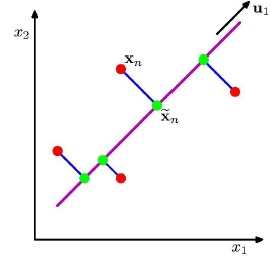
\includegraphics[width=0.3\textwidth]{figures/zASP/projection}
%	\caption{Projection of feature values (red dots) onto PC axes (purple).}
%	\label{projection}
%\end{figure}
%\vspace{-10pt}
%The algebraic method of calculating the PCs can be done by using Singular Value Decomposition (SVD). The first step is to compute the squared cross product matrix of variances and covariances among every pair of the variables in the data set, where the diagonals are the variances and the off-diagonals are the covariances, as done in the following equation \cite{Semmlow2014}:
%%\vspace{-20pt}
%\begin{equation}
%S = X \textquoteright X
%\end{equation}
%Where S is the cross product and X is the feature set matrix. When finding the PCs it includes an eigen-analysis of S. The eigenvalues of are solutions to the following equation \cite{Semmlow2014}:
%%\verticalspace{1}
%\begin{equation}
%| S - \lambda I |  = 0
%\end{equation}
%Where $\lambda$ is the variance of each PC and $I$ is the identity matrix. After solving for $\lambda$ the eigenvectors can be solved through the following equation \cite{Semmlow2014}:
%\begin{equation}
%det | S - \lambda I | b_{i} = 0
%\end{equation}
%Where $b_{i}$ is used to calculate the eigenvectors as in \cite{Semmlow2014}:
%\begin{eqnarray}
%u_{i} = \frac{b_{i}}{\sqrt{b_{i}^{\textquoteright} b_{i}}}
%\end{eqnarray}
%Where $u_{i}$ is the $i^{th}$ number of eigenvectors. The number eigenvectors equal the dimension size of the original feature space. 
%The SVD orders the eigenvalues by size, so that $\lambda_{1} > \lambda_{2} … > \lambda_{i}$. The scores for each PC is equal to the corresponding eigenvalue for that exact axis. The eigenvalues describe how much of the variance is accounted for by the associated PC. Summation of all eigenvalues accounts for the total variance of the data set; this is called the trace. To find how much the each PC accounts for, the eigenvalue of that PC is divided by the total variance: $\%~ of~ total~ variance~ = \frac{\lambda_{i}}{Trace}$. Deciding how many PCs the feature space should be reduced to, by setting a threshold of how much of the total variance should be preserved. \cite{Semmlow2014}

%After reducing the dimensionality of the original feature set the clusters can be analyzed. For the purpose of measuring distances between and within clusters the centroid of each cluster can be calculated, as in \eqref{eq:centroid}:
%
%\begin{equation} \label{eq:centroid}
%	C = \Bigg[ \frac{[x_1+x_2 +~...~+ x_n],[y_1+y_2 +~...~+ y_n] ,~...~,[k_1+k_2 +~...~k_n]}{n} \Bigg]
%\end{equation}
%
%Where $C$ is the centroid, $i$ is the number of feature point in a dimension and $k$ is the number of dimensions. To calculate the distance between centroids of clusters the Euclidean distance (ED) is computed. The ED is the length of the a line segment connecting points, in this case in form of two centroids $p$ and $q$. The calculation of ED in a $k$-dimensional space is as in \eqref{eq:euclidiandistance}:
%
%\begin{equation} \label{eq:euclidiandistance}
%	ED(p,q) = \sqrt{(p_1-q_1)^2 + (p_2-q_2)^2~+~...~+ (p_k-q_k)^2}
%\end{equation} 
%
%When calculating the distance from feature values in a cluster to their corresponding centroid the ED is computed likewise. To get a general impression of the distance from the feature values constituting the cluster to the centroid of the cluster the average of the distances is calculated. 
%
%




